\documentclass{acmsiggraph}                     % final
%\documentclass[annualconference]{acmsiggraph}  % final (annual conference)
%\documentclass[review]{acmsiggraph}            % review
%\documentclass[widereview]{acmsiggraph}        % wide-spaced review
%\documentclass[preprint]{acmsiggraph}          % preprint

%% Uncomment one of the five lines above depending on where your paper is
%% in the conference process. ``review'' and ``widereview'' are for review
%% submission, ``preprint'' is for pre-publication, and ``final'' is for
%% the version to be printed. The ``final'' variant will accept the 
%% ``annualconference'' parameter, which changes the height of the space
%% left clear for the ACM copyright information.

%% The 'helvet' and 'times' packages define the typefaces used for
%% serif and sans serif type in this document. Computer Modern Roman 
%% is used for mathematics typesetting. The scale factor is set to .92
%% to bring the sans-serif type in line with the serif type.

\usepackage[scaled=.92]{helvet}
\usepackage{times}
\usepackage[brazil]{babel}
\usepackage[latin1]{inputenc}

%% The 'graphicx' package allows for the inclusion of EPS figures.

\usepackage{graphicx}

%% use this for zero \parindent and non-zero \parskip, intelligently.

\usepackage{parskip}

%% Optional: the 'caption' package provides a nicer-looking replacement
%% for the standard caption environment. With 'labelfont=bf,'textfont=it',
%% caption labels are bold and caption text is italic.

\usepackage[labelfont=bf,textfont=it]{caption}

%% If you are submitting a paper to the annual conference, please replace 
%% the value ``0'' below with the numeric value of your OnlineID. 
%% If you are not submitting this paper to the annual conference, 
%% you may safely leave it at ``0'' -- it will not be included in the output.

\onlineid{0}

%% Paper title.

\title{Global Illumination for Fun and Profit}

%% Author and Affiliation (single author).

%%\author{Roy G. Biv\thanks{e-mail: roy.g.biv@aol.com}\\Allied Widgets Research}

%% Author and Affiliation (multiple authors).

\author{F�bio Markus Miranda\thanks{e-mail: fmiranda@inf.puc-rio.br}\\ PUC-Rio}

%% Keywords that describe your work.

\keywords{exploded view illustration, interactive visualization}

%%%%%% START OF THE PAPER %%%%%%

\begin{document}

\teaser{
  
\includegraphics[width=1.5in]{sample.png}
  \caption{Lookit! Lookit!}
}

%% The ``\maketitle'' command must be the first command after the
%% ``\begin{document}'' command. It prepares and prints the title block.

\maketitle

%% Abstract section.

\section*{Abstract}
Abstract

\begin{abstract}
Resumo
\end{abstract}

%% ACM Computing Review (CR) categories. 
%% See <http://www.acm.org/class/1998/> for details.
%% The ``\CRcat'' command takes four arguments.

\CRcatlist{
  \CRcat{I.3.5}{Computer Graphics}
  {Computational Geometry \& Object Modeling}{};
  \CRcat{I.3.8}{Computer Graphics}{Applications}{};
}


%% The ``\keywordlist'' command prints out the keywords.
\keywordlist

\section{Introdu��o}
Um problema t�pico na visualiza��o de modelos complexos, como motores, pe�as industriais e dispositivos eletr�nicos, � que as caracter�sticas mais interessantes podem estar obstru�das por outras partes menos importantes. T�cnicas de visibilidade inteligente \cite{Viola-05-Smart} levam em considera��o a relev�ncia dos objetos e suas caracter�sticas, e n�o apenas o seu posicionamento no espa�o, permitindo um maior entendimento do objeto em quest�o.

Uma das t�cnicas de visibilidade � a \emph{vista explodida}, desenvolvida ao longo de s�culos na �rea de ilustra��o t�cnica, e agora utilizada para a visualiza��o de modelos 3D. O seu conceito b�sico � modificar o posicionamento de partes de um modelo para facilitar a vis�o de caracter�sticas importantes. Ao contr�rio de t�cnicas como \emph{ghosted view} e \emph{cut away view}, a vista explodida permite a visualiza��o de um modelo sem que se perca qualquer tipo de informa��o sobre ele, j� que n�o h� nenhum tipo de transpar�ncia ou remo��o de partes mais externas. O usu�rio pode ent�o, baseado em sua experi�ncia, reconstruir mentalmente o modelo e assim ter uma vis�o global e o relacionamento entre as partes que o constituem.

\begin{figure}[h]
	\center{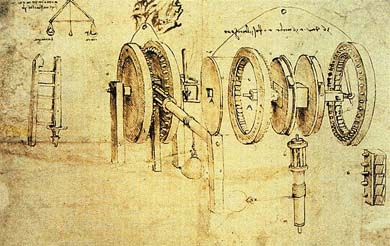
\includegraphics[height=0.5\linewidth]{img/davinci.png}}
	\caption[]{\label{fig:davinci} Exemplo de uma ilustra��o de vista explodida de Leonardo da Vinci.}
\end{figure}

Este trabalho implementa uma t�cnica de vista explodida apresentada em \cite{1360700}. O trabalho busca diminuir a desordem visual ao mesmo tempo que minimiza as dist�ncias de explos�o, facilitando assim o entendimento das rela��es entre as partes do modelo. Para isso, � proposto a constru��o de um \emph{grafo de explos�o}, que ir� ditar a ordem e a dire��o com que cada parte poder� ser explodida. O usu�rio poder� escolher quais partes deseja visualizar e o sistema ir� expandir (ou colapsar) de acordo com o que foi previamente gerado no grafo.

O objeto principal aqui � dar uma vis�o geral sobre o tema, explicar o trabalho escolhido, assim como a sua implementa��o, discutir dificuldades e facilidades e apresentar poss�veis propostas para trabalhos futuros.

Este trabalho est� dividido da seguinte forma: na Se��o \ref{trabalhosrelacionados} s�o apresentados os trabalhos relacionados. A Se��o \ref{metodologia} apresenta uma vis�o geral do sistema de vista explodida, sendo que detalhes de implementa��o s�o discutidos na Se��o \ref{implementacao}. Os resultados s�o mostrados na Se��o \ref{resultados}. A conclus�o e poss�veis trabalhos futuros est�o na Se��o \ref{conclusao}.
\section{Trabalhos Relacionados}
\label{trabalhosrelacionados}

\begin{figure*}
	\center{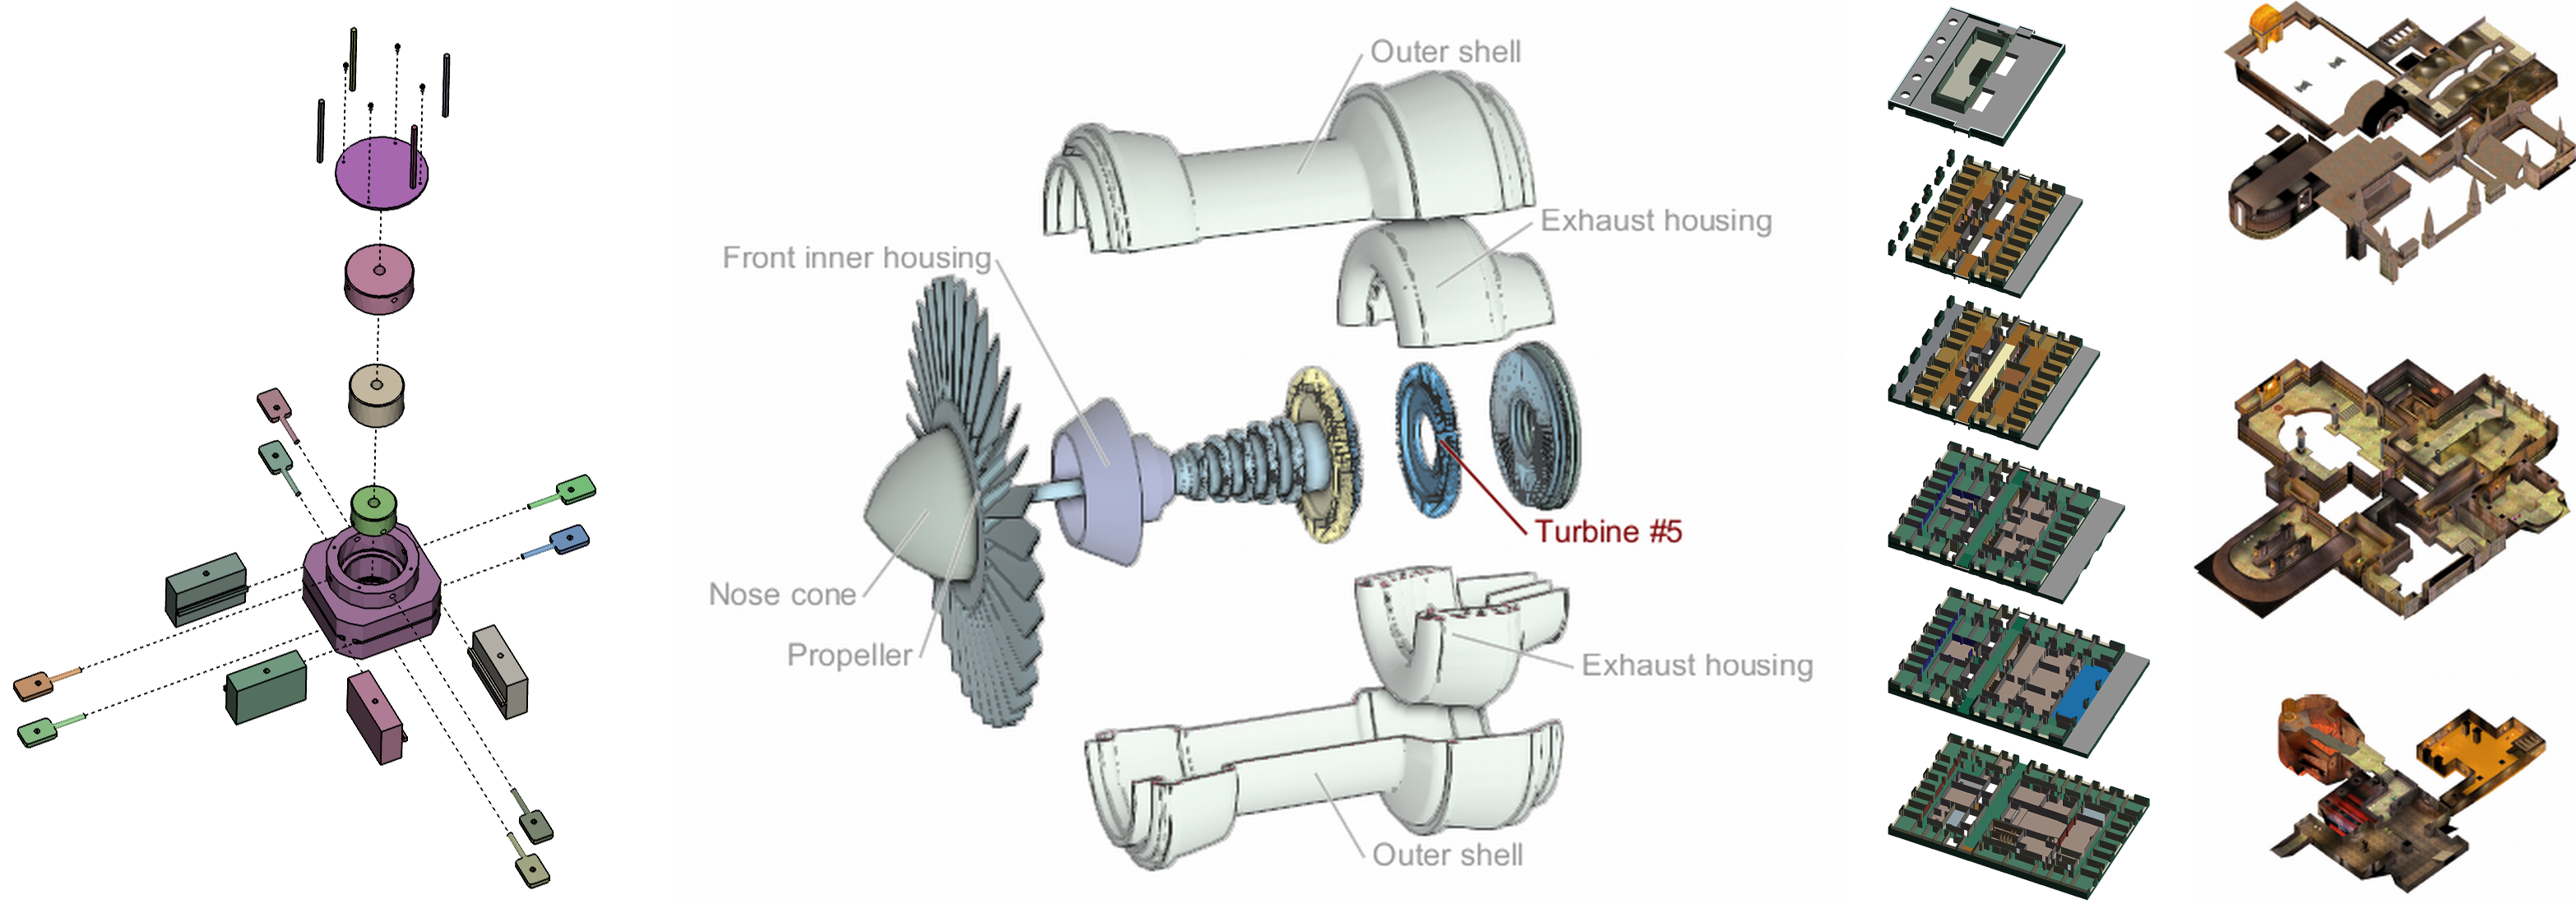
\includegraphics[width=1.0\linewidth]{img/trabalhosrelacionados2.png}}
	\caption[]{\label{fig:trabalhosrelacionados} Trabalhos relacionados (\cite{857608}, \cite{1081497}, \cite{1187828}, \cite{882352}, \cite{1360700}, \cite{641493}, \cite{1271635}).}
\end{figure*}

O trabalho apresentado em \cite{Viola-05-Smart} faz um levantamento de diversas t�cnicas desenvolvidas com o objetivo de facilitar a visualiza��o de modelos complexos e, por ser bastante abrangente, serve como uma base para o estudo da �rea. Em \cite{1446259}, os autores apresentam cinco \emph{patterns} (como \emph{tour planner, interactive exploder, virtual X-Ray, etc}), derivados de 25 caracter�sticas, com o objetivo de classificar diferentes t�cnicas de gerenciamento de oclus�o, apresentando os pontos positivos e negativos de cada uma. Segundo o artigo, a vista explodida possui a vantagem de n�o remover nenhum tipo de informa��o do modelo e tamb�m mant�m todas as suas informa��es de relacionamento, ao contr�rio das t�cnicas baseadas, por exemplo, em \emph{cut outs}.

Os trabalhos relacionados a vista explodida podem ser divididos em dois grupos. Uma primeira s�rie de trabalhos busca criar vistas explodidas com base em dados volum�tricos. O primeiro a explorar essa �rea foi \cite{857608}, onde os autores descrevem a t�cnica \emph{visual access distortion}, que busca criar um caminho de visualiza��o sem obstru��es at� a parte de maior interesse. Por�m, a t�cnica, como descrita originalmente, aumenta o tamanho das partes mais importantes do modelo, o que pode distorcer qualquer tipo de relacionamento espacial entre as partes. Os trabalhos \cite{1187828} e \cite{1081497} tamb�m apresentam propostas para a visualiza��o de dados volum�tricos com vistas explodidas, mas sem nenhum tipo de deforma��o. Os resultados s�o aplicados na visualiza��o de dados volum�tricos de car�ter m�dico.

Uma outra vertente na pesquisa de vistas explodidas � voltado para a explos�o de modelos 3D complexos, n�o baseados em dados volum�tricos. O trabalho \cite{882352} � uma refer�ncia inicial nesse assunto e apresenta um sistema para gera��o de instru��es de montagem, mas n�o prop�e nada relacionado a vistas explodidas em espec�fico. Esse tema s� � abordado no artigo \cite{1360700}, que busca justamente expandir as instru��es de montagem e criar um sistema para a visualiza��o de vistas explodidas, dada a semelhan�a entre os dois assuntos. Esse �ltimo trabalho tamb�m � integrado ao trabalho \cite{2667077}, onde � apresentado um sistema de \emph{cut away view}.

Outro trabalho tamb�m relacionado a vistas explodidas � \cite{641493}, onde os autores apresentam um sistema para a gera��o autom�tica de vistas explodidas de constru��es, levando em considera��o as normais do modelo e a altura m�dia dos andares. Como resultado, os autores mostram a utiliza��o do sistema na navega��o interativa em ambientes arquitet�nicos e tamb�m em jogos \emph{online}, onde o "telespectador" pode ter uma vis�o global dos diferentes andares de um mapa de um jogo.

Finalmente, o trabalho \cite{1271635} utiliza t�cnicas de vista explodida n�o para visualizar modelos 3D, mas para visualizar dados, como a classifica��o taxon�mica de animais.

A Figura \ref{fig:trabalhosrelacionados} apresenta algumas imagens dos trabalhos na �rea de vistas explodidas.
\section{Implementa��o}

\begin{frame}\frametitle{Implementa��o}
\begin{itemize}
	\item OpenSceneGraph para a renderiza��o e carregamento dos modelos.
	\item PQP para a detec��o de colis�o entre as partes.
\end{itemize}
\end{frame}



\begin{frame}\frametitle{Implementa��o}
\begin{itemize}
	\item Vis�o geral:
	\begin{columns}[T]
	\begin{column}{2cm}
	\begin{overprint}
		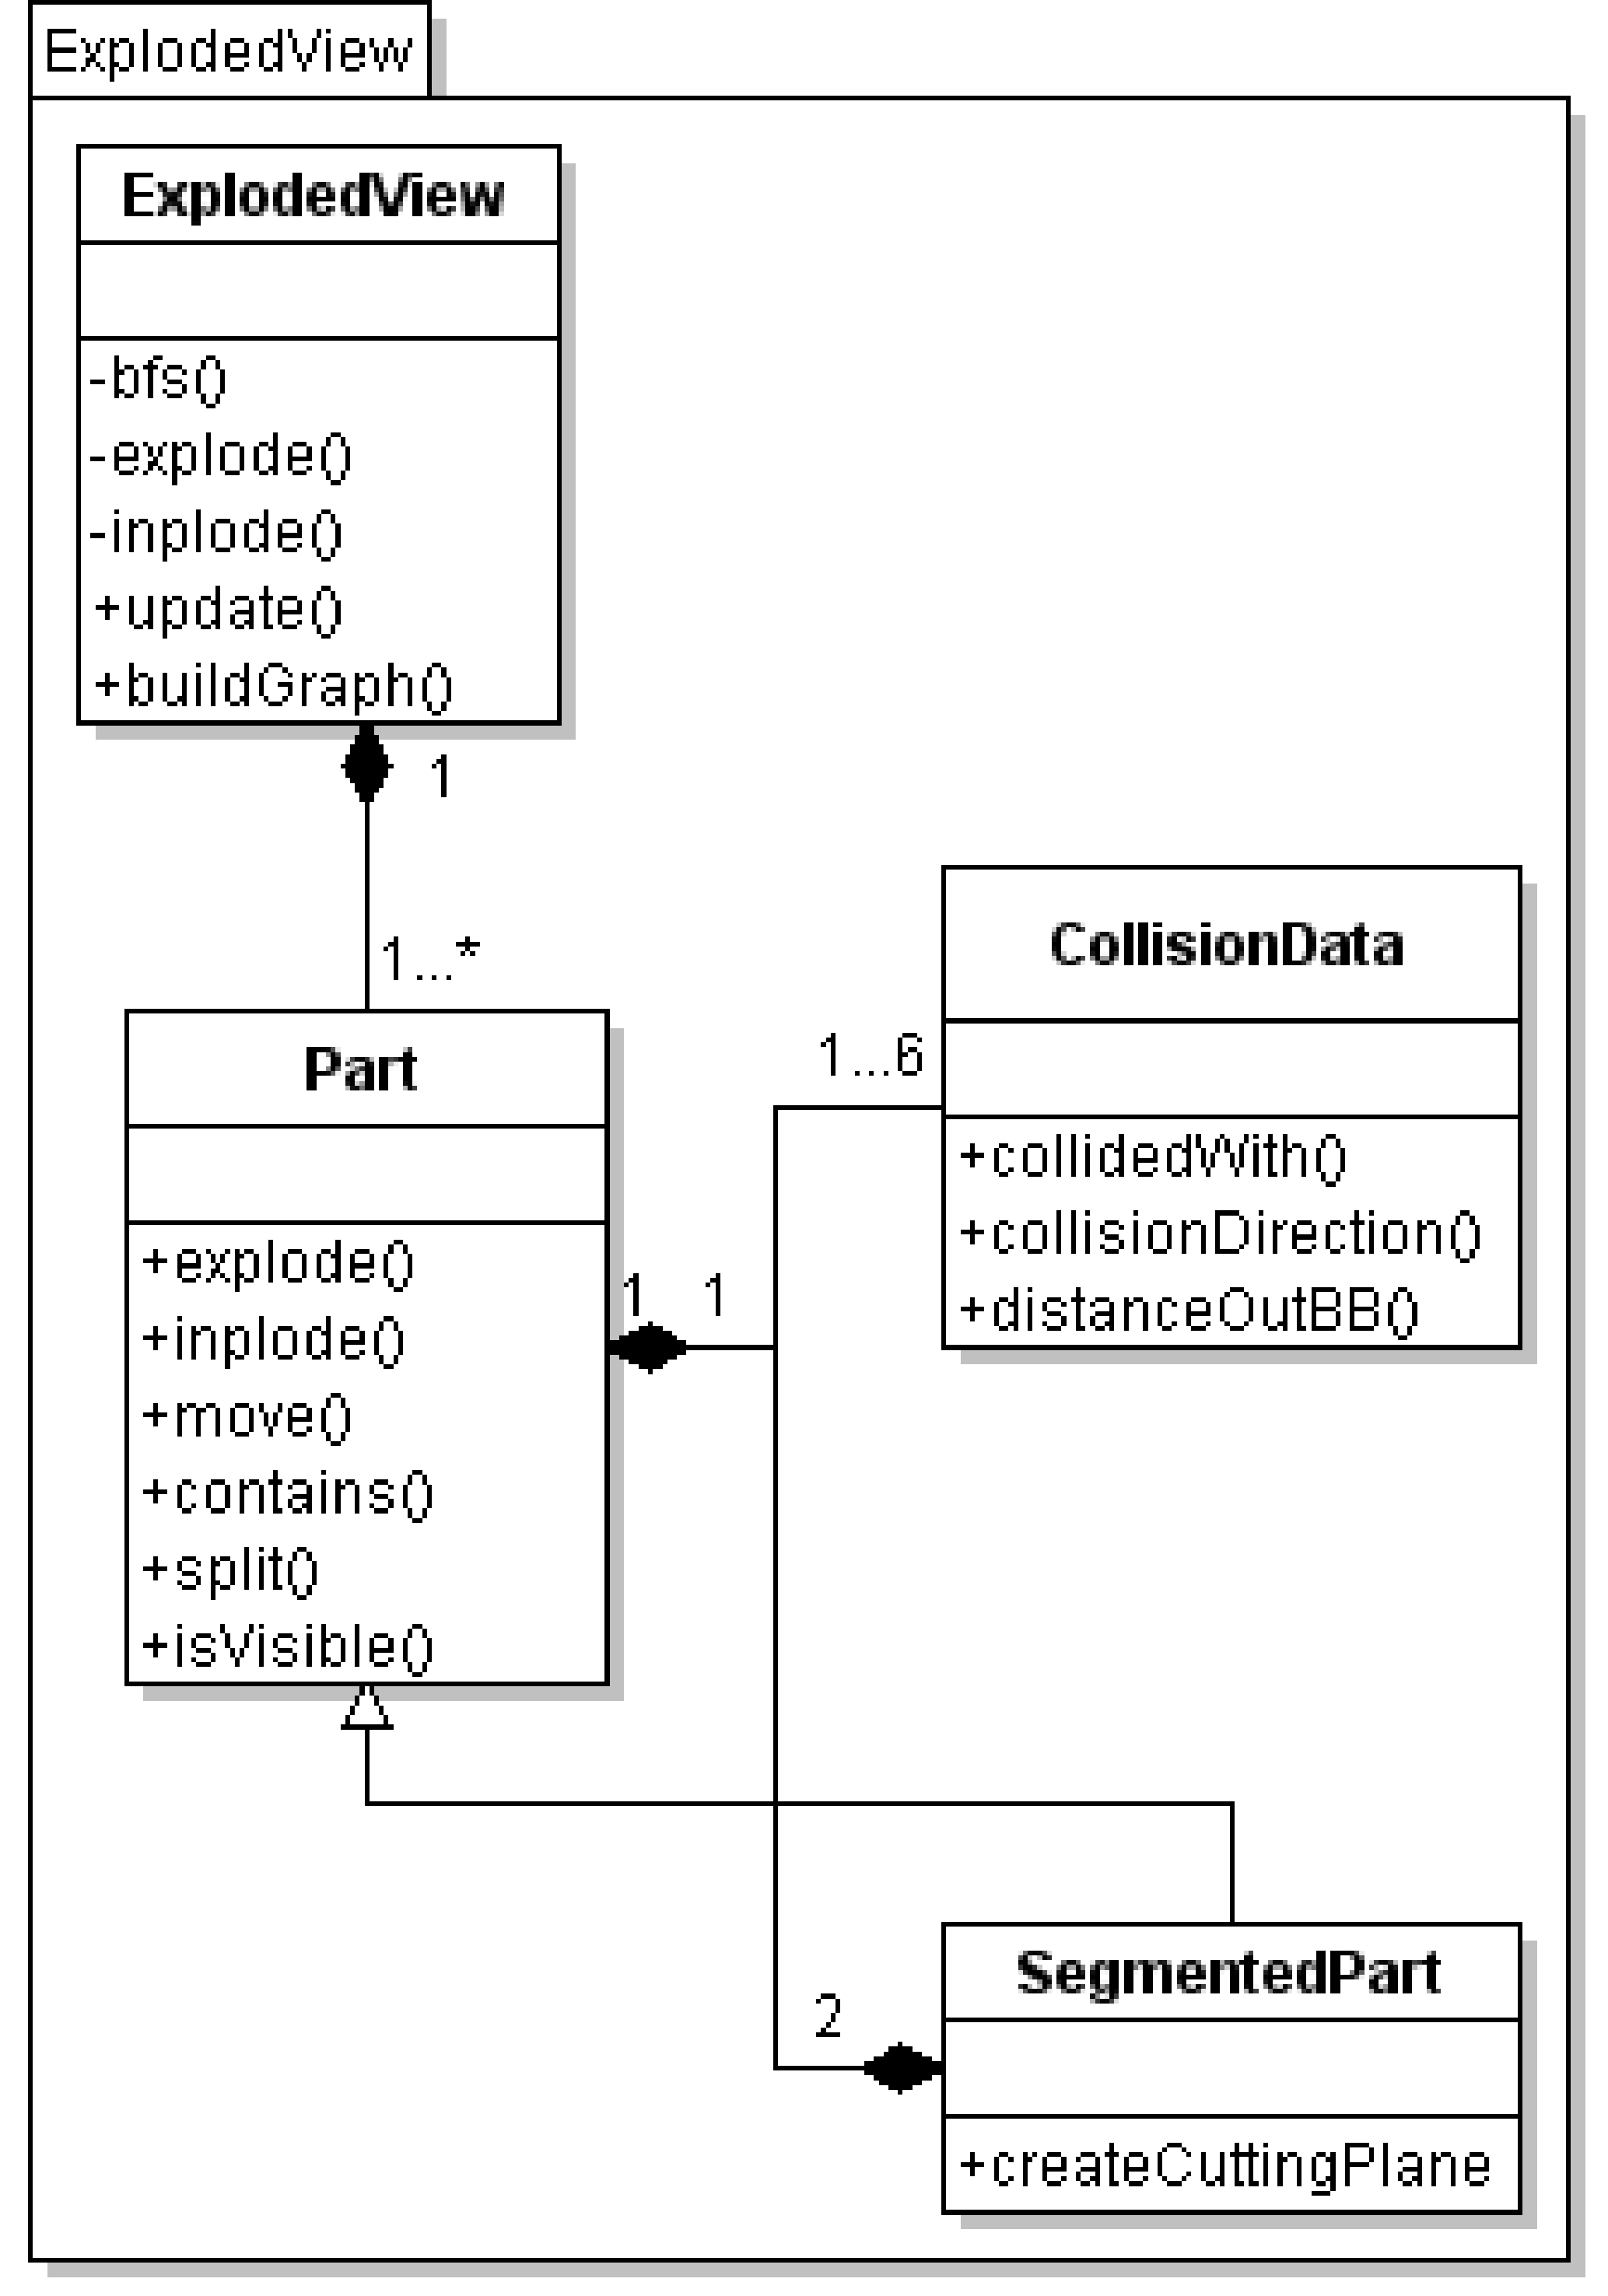
\includegraphics[height=150.0px]{img/arquitetura}
	\end{overprint}
	\vspace{3cm} 
	\end{column}
	\begin{column}{5cm}
	\begin{itemize}
		\item \footnotesize \textbf{ExplodedView}: classe geral, respons�vel pelo por tratar os dados de entrada (tanto o modelo 3D quanto o \emph{input} do usu�rio).
		\item \footnotesize \textbf{Part}: classe que representa as partes do modelo.
		\item \footnotesize \textbf{SegmentedPart}: classe que herda de \textbf{Part} e representa os recipientes divididos. A divis�o dos modelos � feita atrav�s de um \textbf{ClipNode} do \textbf{OSG}.
		\item \footnotesize \textbf{CollisionData}: representa os dados de colis�o.
	\end{itemize}
	\end{column}
	\end{columns}
\end{itemize}
\end{frame}

\begin{frame}\frametitle{Implementa��o}
\center 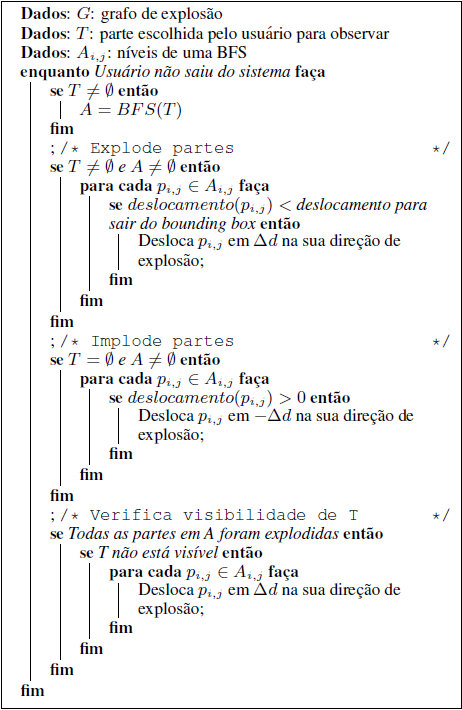
\includegraphics[height=200.0px]{img/algoritmo}
\end{frame}
\section{Resultados}
Resultados
\section{Conclus�o e Trabalhos Futuros}
\label{conclusao}
O artigo \cite{1360700}, com sua proposta de grafos de explos�o, apresenta uma boa maneira para a visualiza��o de modelos 3D, uma vez que essa representa��o � uma forma ideal e bastante intuitiva de relacionar diferentes partes e o bloqueio existente entre cada uma delas. As principais caracter�sticas foram implementadas neste trabalho; alguns pontos foram simplificados, mas isso n�o comprometeu o resultado final, j� que o principal ponto, a explos�o das partes, foi implementado satisfatoriamente, com bons resultados para os modelos de teste.

Al�m do estudo do artigo citado, este trabalho se mostrou muito �til para adquirir um conhecimento maior na �rea de t�cnicas de visibilidade inteligente e os problemas que cada t�cnica busca solucionar.

Um grande problema durante o desenvolvimento foi a falta de modelos 3D para o teste do sistema. Apesar dos modelos criados representarem bem as caracter�sticas e recursos do sistema, eles certamente possuem uma complexidade bem inferior aos modelos 3D reais, seja na quantidade de partes ou na disposi��o das mesmas. O pr�prio artigo cita que o sistema pode ter resultados insatisfat�rios para modelos com superf�cies com algum tipo de irregularidade.

Um problema que pode ser explorado � a explos�o de pe�as ao longo de um conjunto de eixos, possibilitando que modelos mais complexos sejam explodidos. Como a reconstru��o mental do modelo por parte do usu�rio pode ficar comprometida, outros recursos gr�ficos poderiam ser estudados, como linhas ligando a posi��o original da parte at� o seu destino. Outro aspecto � a divis�o do modelo 3D em partes. O artigo que este trabalho implementou j� considera que o modelo de entrada est� bem dividido, algo que n�o ocorre necessariamente.

Al�m disso, o uso de vista explodida para a visualiza��o de dados e informa��o (como \cite{1271635}), e n�o s� para modelos 3D convencionais, parece ser promissor.

Finalmente, poucos trabalhos buscam unir diferentes t�cnicas de visualiza��o inteligente e avaliar os resultados e a facilidade de interpreta��o do modelo. Um caminho seria avaliar se tal uni�o realmente � vantajosa e como ela poderia ser feita. O uso de realidade aumentada tamb�m poderia ser estudado, como forma de auxiliar a intera��o do usu�rio com as diversas partes que formam um modelo 3D.


%\section*{Acknowledgements}

%To Robert, for all the bagels.

\bibliographystyle{acmsiggraph}
\nocite{*}
\bibliography{paper}
\end{document}
